% start of file `cv_german.tex', based on `template_en.tex`
% by Xavier Danaux (xdanaux@gmail.com).
% This work may be distributed and/or modified under the
% conditions of the LaTeX Project Public License version 1.3c,
% available at http://www.latex-project.org/lppl/.
%
% Thomas Quaritsch <t.quaritsch@student.tugraz.at>

\documentclass[11pt,a4paper]{moderncv}

% \usepackage[german]{babel}
\usepackage[english]{babel}
\usepackage[utf8]{inputenc}
\usepackage{multicol}
\moderncvtheme[blue]{casual}
\usepackage{moderncv-additions}

% adjust the page margins
\usepackage[scale=0.8]{geometry}
\setlength{\hintscolumnwidth}{3cm}

% if you want to change the width of the column with the dates
% \AtBeginDocument{\setlength{\maketitlenamewidth}{6cm}}
% only for the classic theme, if you want to change the width
% of your name placeholder (to leave more space for your address details

\AtBeginDocument{\recomputelengths}
% required when changes are made to page layout lengths

% personal data
\firstname{Philipp}
\familyname{Hacker}
\address{Erich-Böhmke-Straße 22a}{17489 Greifswald}
\mobile{+49 1520 209 5 226}
\email{rayleighsjeans@gmail.com}
\photo[64pt]{picture}

% \title{Resumé title (optional)}
% \phone{phone (optional)}
% \fax{fax (optional)}
% \extrainfo{additional information (optional)}

% '64pt' is the height the picture must be resized
% to and 'picture' is the name of the picture file
% \quote{``Das ist ein toller Frusterspruch\\%
%      von Friede Frusterfrau.'' -- Friede Frusterfrau}

% \nopagenumbers{}
% uncomment to suppress automatic page numbering for CVs
% longer than one page

\newcommand{\sign}[1]{%
  \begin{tabular}[t]{@{}l@{}}
  \makebox[1.5in]{\dotfill}\\
  \strut\emph{#1}\strut%
  \end{tabular}}%
\newcommand{\position}{%
    Softwareentwickler Windows (w/m/d)}

%-------------------------------------------------------------------------------
%            content
%-------------------------------------------------------------------------------
\begin{document}

    % color redefinitions must be after \begin{document}!
    \definecolor{firstnamecolor}{RGB}{138,74,57}
    \definecolor{familynamecolor}{RGB}{138,74,57}
    \definecolor{quotecolor}{RGB}{125,85,85}
    \definecolor{addresscolor}{RGB}{125,85,85}
    \definecolor{sectionrectanglecolor}{RGB}{138,74,57}
    \definecolor{sectiontitlecolor}{RGB}{138,74,57}
    \definecolor{subsectioncolor}{RGB}{125,85,85}
    \definecolor{footersymbolcolor}{RGB}{125,85,85}

    \makeatletter
    \pagestyle{empty}
    \chapter*{Application}{~Form}

    \vspace*{3.5cm}
    \begin{minipage}{\textwidth}
        \vspace*{3mm}
        \familynamestyle{\@firstname}~\firstnamestyle{\@familyname}
            \hspace*{5mm}%
            {{\color{firstnamecolor}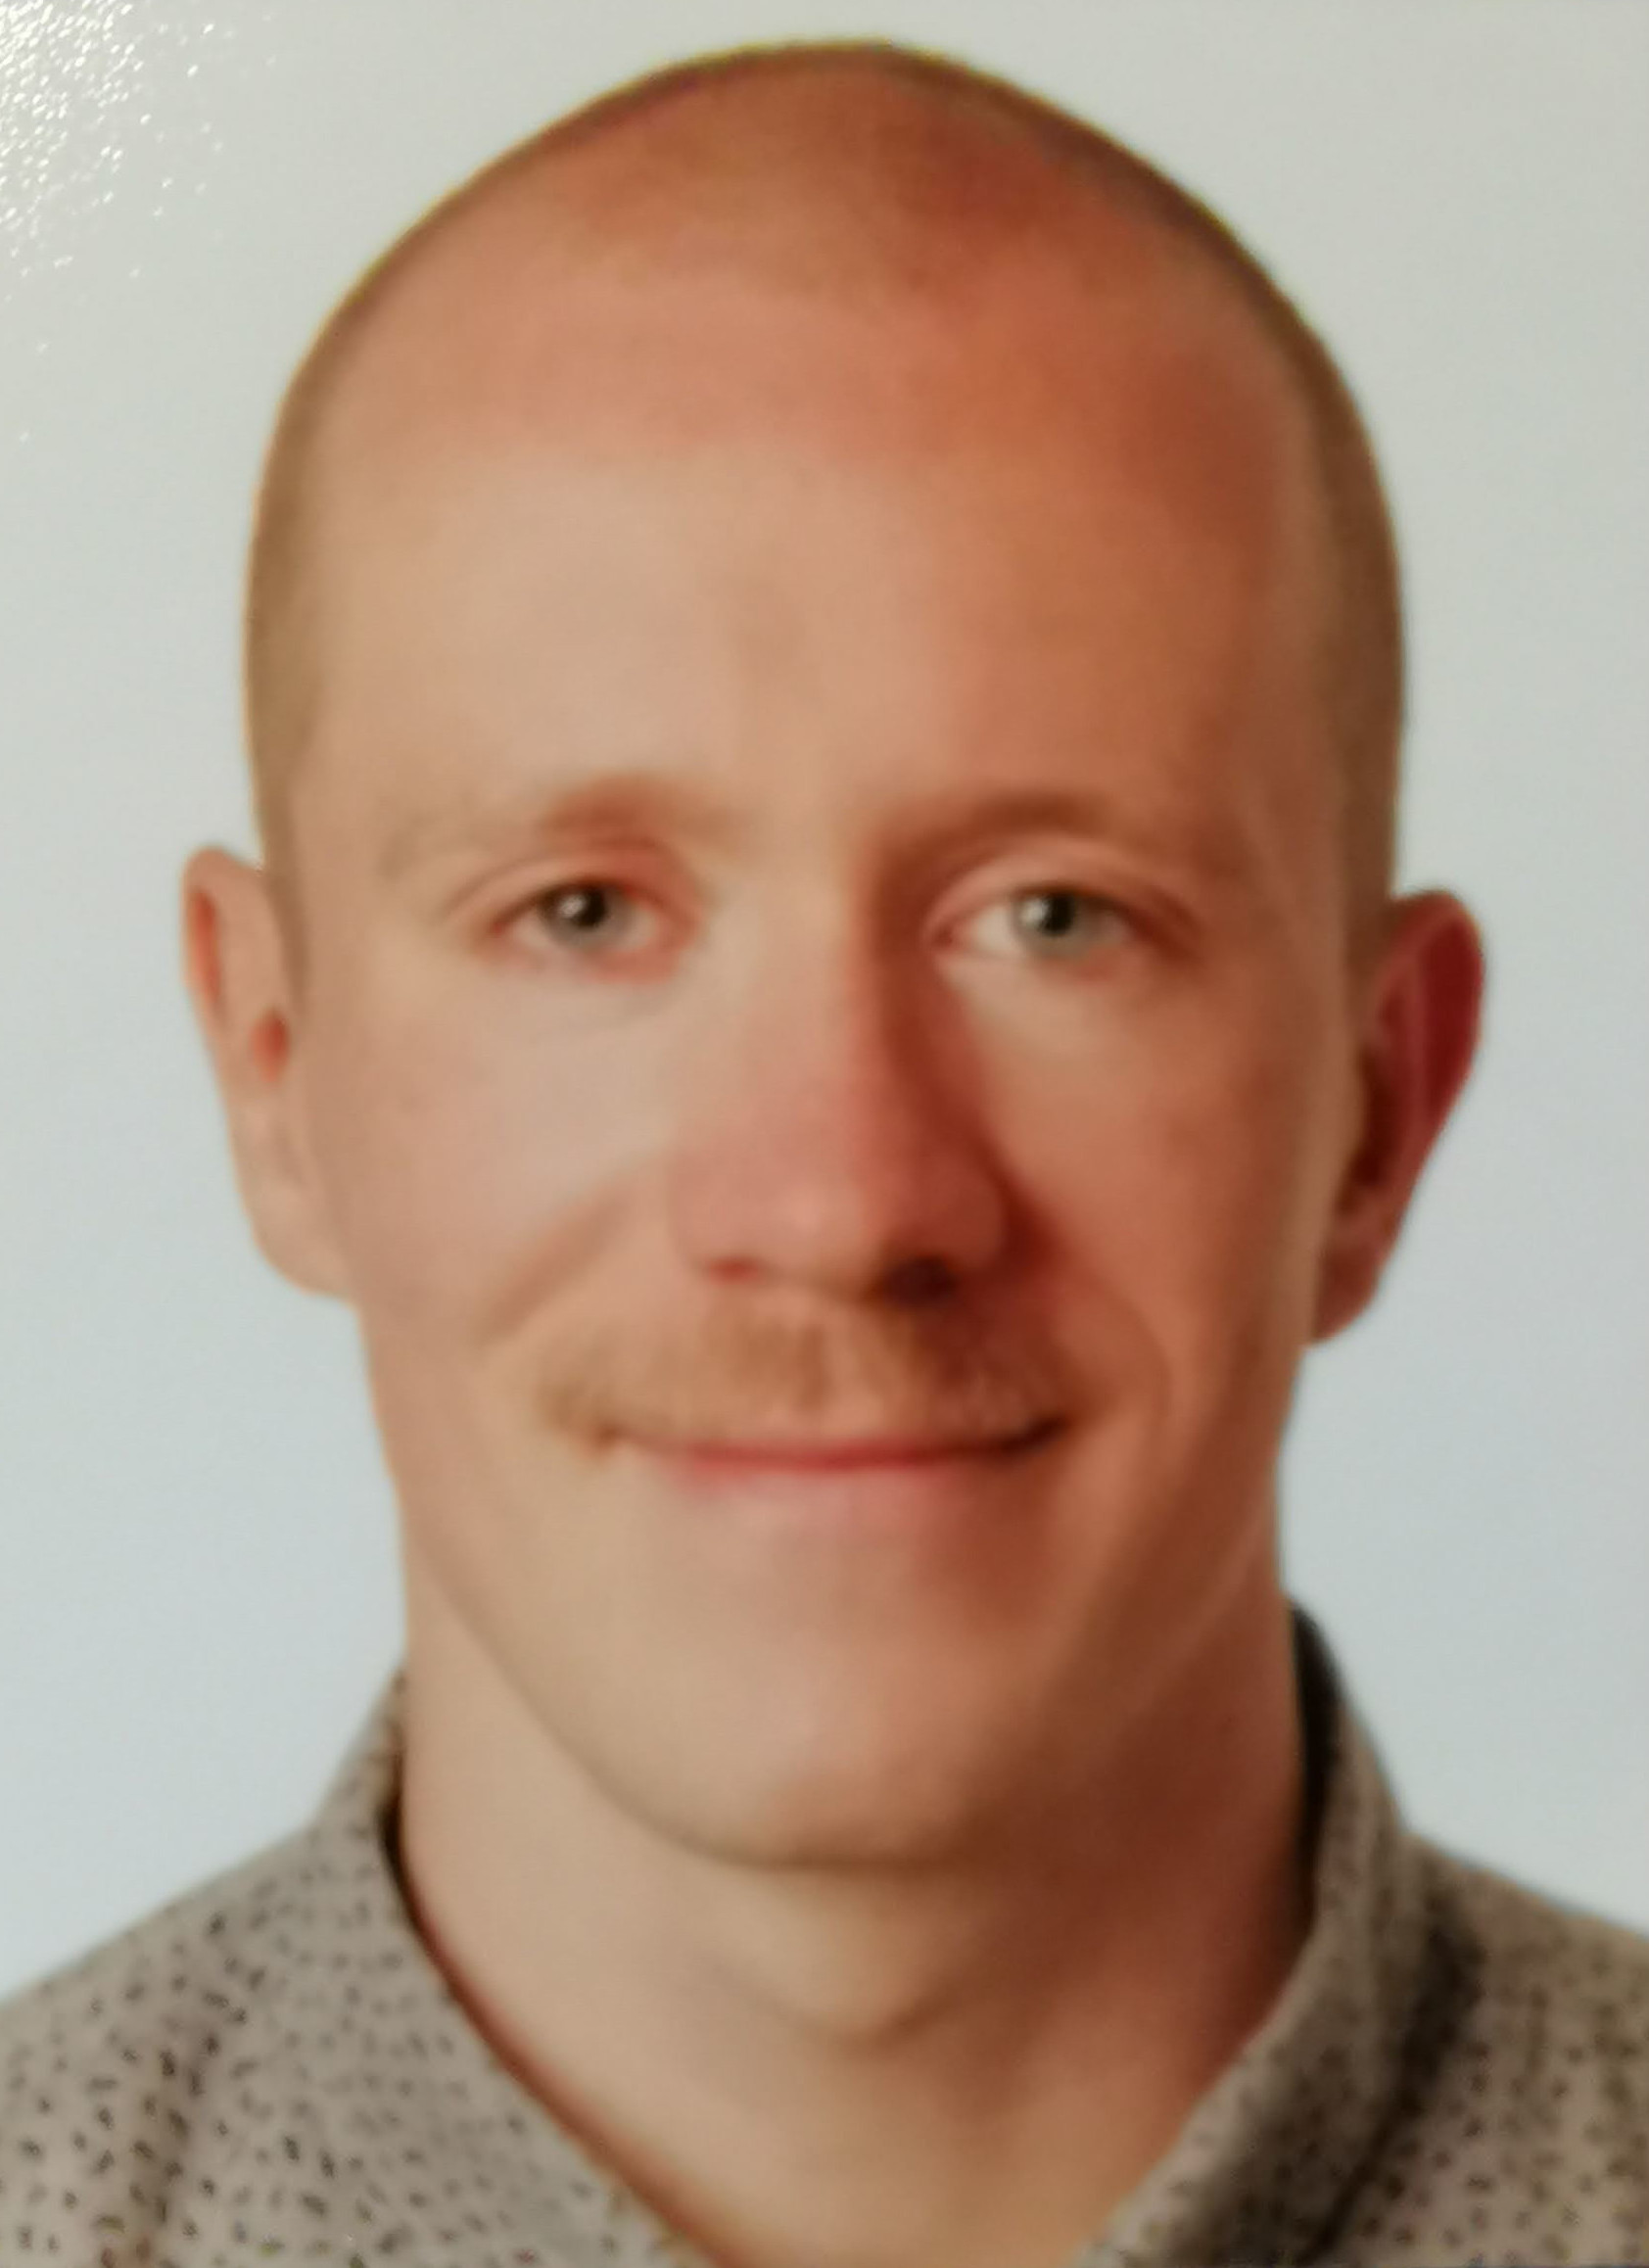
\includegraphics[width=96pt]{%
                ../figures/images/42.jpg}}}\\[0.3cm]
            \@addressstreet\\[0.0cm]%
            \@addresscity\\[0.3cm]%
            \mobilesymbol~\@mobile\\[0.3cm]%
            \emailsymbol~\@email%
    \end{minipage}
    \begin{minipage}{70pt}
    \end{minipage}
    % \vfill
    % \begin{minipage}{1.0\textwidth}
    %     \section{Contents}
    %     \tableofcontents
    % \end{minipage}

    %---------------------------------------------------------------%
    %            letter
    %---------------------------------------------------------------%
    \newpage
    \makeatletter
    \chapter{Application}{~Letter}

    \vspace*{1.0cm}
    \begin{minipage}{0.6\textwidth}
        \begin{flushleft}
            % {\bfseries{\color{firstnamecolor}%
            %     Stelle\\[0.1cm]%
            %     Position
            % }}\\[0.2cm]
            Thermo Fisher Scientific Inc.\\%
            Personalstelle, Ref.: 133730BR\\%
            Germering, Germany
        \end{flushleft}
    \end{minipage}
    \hfill
    \begin{minipage}{0.3\textwidth}
        \begin{flushright}
            % \vspace*{1.3cm}
            Philipp Hacker\\%
            Erich-Böhmke-Straße 22a\\%
            17489 Greifswald
            \today
        \end{flushright}
    \end{minipage}

    \vspace*{1.0cm}
    {\bfseries \color{familynamecolor}%
        Application~for~\position\\
    }\\[0.75cm]
%
    Dear Mrs.\ or Mr.,\\[0.75cm]%
%
    with this form I would like to submit my initial application for the position of~\position.\\[0.75cm]  % TODO
%
        I am currently working on my PhD thesis under the supervision of Prof. Dr. Thomas Klinger at the Max-Planck Institute for Plasma Physics in Greifswald. I am expected to finish my PhD with the submission and defense of my thesis in mid to late april of 2021.\\[0.75cm]%
%
        Over the course of my study and PhD I had the chance to acquire experiences in different fields of computational science, ranging from simulation, optimisation and controlling to integration. Additionally, I was able to learn about and apply the first steps towards the implementation of machine learning. Especially during my PhD I had the opportunity to work hands-on the design, conceptioning and execution of a complex forward-feedback controll system of a plasma diagnostic. My curiosity and passion for intelligent solutions to complex challenges motivates me for an application in new fields.\\[0.75cm]%
%
        At last I will note the names and contact info of my previous supervisors as references.\\[0.5cm]
        \hspace*{0.5cm}Prof. Dr. Andre Melzer (Colloidal Plasma)%
            \hfill Tel. +49~3834~/~420~4790\\
        \hspace*{0.5cm}Prof. Dr. Ralf Schneider (Computational Science)%
            \hfill Tel. +49~3834~/~420~1400\\
        \hspace*{0.5cm}Prof. Dr. Thomas Klinger (E5 - Divertor Dynamics and Transport)%
            \hfill Tel. +49~3834~/~~\,88~2500\\
%
    \vspace*{0.2cm}
    \begin{flushleft}
        Yours sincerely,\\[0.75cm]
        \vspace*{-1.0cm}%
        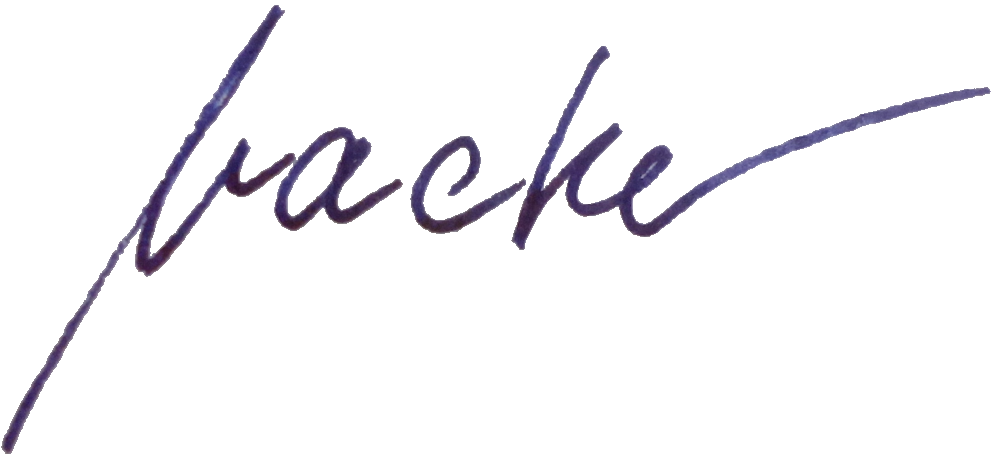
\includegraphics[width=4.0cm]{%
            ../figures/images/signature_transparent.png}
        \hspace*{-4.0cm}\sign{Philipp Hacker}\\[0.0cm]
        % Greifswald; \today
    \end{flushleft}
%
    % \newpage
    % \pagestyle{fancy}
    % \chapter{Curriculum}{~Vitae}
    % \makequote%

    % %/******************************************************************/%
    % \section{Personal~Information}
    % \cvline{Name}{\@firstname~\@familyname}
    % \cvline{Address}{\@addressstreet\newline \@addresscity}
    % \cvline{Telephone}{\@mobile}
    % \cvline{eMail}{\@email}
    % \cvline{Date~of~Birth}{15th~of~June,~1994~in~Demmin}
    % \cvline{Nationality}{Germany}
    % \cvline{Family~Status}{unwed}
    % \cvline{Sex}{Male}
    % % \cvline{Präsenzdienst}{abgeleistet}
    % % \cvline{Führerschein}{A,B,C,D,E,F,G}
    % \makeatother

    % % \cventry{1901--1902}{Degree}{Institution}{City}%
    % %	 	 {\textit{Grade}}{Description}
    % % arguments 3 to 6 are optional

    % %/******************************************************************/%
    % \section{Languages}
    % \cvline{German}{first language, mother tongue}{}
    % \cvline{English}{second language, first foreign lingo\newline 7 years of school education}{}
    % \cvline{Russian}{third language, second foreign lingo\newline 5 years of school education}{}

    % %/******************************************************************/%
    % \section{School}
    % \cventry{08/2000--03/2004}{Elementary~School}{Grundschule~Jarmen\newline~Jarmen}{}{}{}
    % \cventry{08/2004--08/2010}{Middle~School}{Regionale~Schule~Jarmen\newline~Jarmen}{}{}{}
    % \cventry{08/2010--06/2012}{Academic~High~School}{%
    %         Schlossgymnasium Gützkow,~Gützkow\newline}{}%
    %     {Higher~Education~Entrance~Qualification\newline}{%
    %         (Certificate~included)}

    % %/******************************************************************/%
    % \section{Higher Education}
    % \cventry{10/2012--09/2015}{Bachelors~Degree~in~Physics}{%
    %         Ernst-Moritz-Arndt~University}%
    %     {Greifswald}{Bachelor~of~Sciences}{%
    %         (Certificate~and~course~overview~included)}
    % \cventry{10/2012--~20/2017}{Masters~Degree~in~Physics}{%
    %         Ernst-Moritz-Arndt~University}%
    %     {Greifswald}{Master~of~Sciences}{%
    %         (Certificate~and~course~overview~included)}
    % %/******************************************************************/%
    % \newpage
    % \section{Research Experience}
    % \cventry{10/2012--04/2014}{Basic~Practical~Laboratory~Course}%
    %     {Basic~experiments~in~all~research~fields~at~the~Institute~of~Physics\newline}{}%
    %     {University~of~Greifswald}{}
    % \cventry{05/2015--09/2015}{%
    %         Bachelor~Thesis:~`Modenanregung~in~Yukawa-Bällen'}%
    %     {Research~Group~of~Prof.~Dr.~Andre~Melzer\newline}{}%
    %     {University~of~Greifswald\newline}{Stereoscopic particle diagnostics with MATLAB}
    % \cventry{10/2015--07/2016}{Intership~in~the~Group~of~Prof.~Dr.~Melzer}%
    %     {Complex~Plasma~Systems,~Experiment~Setup\newline}{}%
    %     {Institute~of~Physics,~University~of~Greifswald}{}
    % \cventry{10/2015--04/2016}{Advanced Practical Laboratory Course}%
    %     {Advanced experimental methodology\newline}{}%
    %     {Institute~of~Physics,~University~Greifswald}{}
    % \cventry{04/2016--10/2016}{Research~Group~Internship}%
    %     {`Electric~field~strength~spectroscopy~in~dielectric~barrier~discharges'\newline}{}%
    %     {Research~Group~of~Prof.~Dr.~Jürgen~Meichsner\newline}%
    %     {Institute~of~Physics,~University~of~Greifswald}
    % \cventry{10/2016--10/2017}{%
    %     Master~Thesis:~`Kinetic~Effects~in~RF~Discharges'}%
    %     {Research~Group~of~Prof.~Dr.~Ralf~Schneider\newline}{}%
    %     {Institute~of~Physics,~University~of~Greifswald\newline}%
    %     {C++ 2d3v PIC simulation of ccrf discharges}
    % \cventry{11/2017--now}{%
    %     International~Helmholtz~Graduate~School~for~Plasma~Physics}%
    %     {Graduate~School~for~Doctoral~Candidates~at~the~MPI~for~Plasma Physics\newline}{}%
    %     {MPI~for~Plasma~Physics,~Greifswald;~University~of~Greifswald\newline}%
    %     {presentations~and~participation~in~colloquia,~workshops~and~conferences}
    % \cventry{11/2017--now}{%
    %     PhD:~`Impurity~radiation~and~transport~at~the~stellarator~Wendelstein~7-X'}%
    %     {Division~of~Stellarator~Dynamics~and~Transport,~Prof.~Dr.~T.~Klinger\newline}{}%
    %     {Max-Planck~Institute~for~Plasma~Physics,~Greifswald\newline}%
    %     {real~time~feedback~on~plasma~radiation,~evaluation~of~local~radiation~sensitivity}

    % %/******************************************************************/%
    % \section{Lecturing Experiences}
    % \cventry{2014-2018}{Assistant~Associate~in~the~Practical~Course~-~Physics}%
    %     {in:~Study~Programme~of~Humane~Medicine\newline}{}%
    %     {Institute~of~Physics,~University~of~Greifswald}{}

    % %/******************************************************************/%
    % \section{Publications}
    % \cventry{May~2018}{%
    %         `PIC~Simulation~of~electronegative~CCRF~discharges'}%
    %     {Authors:~P.~Matthias,~R.~Schneider,~J.~Meichsner,~%
    %      G.~Bandelow,~J.~Duras,~K.~Matyash, K.-F.~Lüskow,~D.~Kahnfeld,~%
    %      S.~Kemnitz,~L.~Lewerentz~and~P.~Hacker}{%
    %         doi:~10.1140/epjd/e2017-80565-y}{}{}
    % \cventry{Dec.~2019}{%
    %         `Measurement of edge ion temperature in W7-X with island divertor by retarding field analyzer'}%
    %     {Authors:~Y.~Li,~.~ Henkel,~Y.~Liang,~A.~Knieps,~P.~Drews,~C.~Killer,~D.~Nicolai,~J.~Cosfeld,~J.~Geiger,~Y.~Feng,~F.~Effenberg,~D.~Zhang,~P.~Hacker,~D.~Höschen,~G.~Satheeswaran,~S.~Liu,~O.~Grulke,~M.~Jakubowski, S.~Brezinsek,~M.~Otte,~O.~Neubauer,~B.~Schweer1,~G.~S.~Xu,~J.~Cai,~Z.~Huang,~the W7-X~Team}{doi:~10.1088/1741-4326/ab3a79}{}{}
    % \cventry{Jul.~2019}{%
    %         `The~influence~of~impurity~radiation~locations~on~the~plasma~performance~in~stellarator~Wendelstein~7-X'}%
    %     {Authors:~D.~Zhang,~R.~Burhenn,~F.~Reimold,~P.~Hacker,~L.~Giannone,~K.~J.~Brunner,~B.~Buttenschön,~G.~Fuchert,~H.~P.~Laqua,~K.~Rahbarnia,~C.~D.~Beidler,~S.~Brezinsek,~Y.~Feng,~M.~Jakubowski,~R.~König}{}{}{}
    % \cventry{Feb.~2020}{%
    %         `Absence~of~Non-Local~Electron~Heat~Transport~in~ASDEX~Upgrade~and~Wendelstein~7-X~and~Modelling
    %         ~with~the~Transport~Code~ASTRA'}%
    %     {Authors:~K.~Höfler,~T.~Happel,~P.~Hennequin,~U.~Höfel,~F.~Ryter,~U.~Stroth,~A.~Bock,~P.~David,~S.~Denk,~A.~Dinklage,~G.~Fuchert,~P.~Hacker,~M.~Hirsch,~P.~A.~Schneider,~J.~Schilling,~T.~Stange,~G.~Tardini,~T.~Andreeva,~M.~Beurskens,~S.~Bozhenkov,~K.~J.~Brunner,~N.~Chaudhary,~H.~Damm,~U.~Neuner,~J.~W.~Oosterbeek,~E.~Pasch,~K.~Rahbarnia,~H.~Thomsen, M.~Zanini,~D.~Zhang,~the~ASDEX~Upgrade~Team,~the~Wendelstein~7-X~Team}{}{}{}
    % \cventry{Feb.~2020}{%
    %         `Large wetted areas of divertor power loads at Wendelstein 7-X'}%
    %     {Authors:~H.~Niemann,~P.~ Drewelow,~M.~ Jakubowski,~A.~Puig Sitjes,~B.~Cannas,~Y.~Gao,~F.~Pisano,~R.~König,~R.~Burhenn,~P.~Hacker,~F.~Reimold,~D.~Zhang,~K.~J.~Brunner,~J.~Knauer,~T.~Sunn~Pedersen}{%
    %     doi:~10.1088/1741-4326/ab937a}{}{}
    % \cventry{unreleased,~exp.~2021}{%
    %         `Stellarator-Tokamak~Energy~Confinement~Comparison~based~on~ASDEX~Upgrade~and~Wendelstein~7-X~Hydrogen~Plasmas'}%
    %     {Authors:~U.~Stroth,~G.~Fuchert,~M.~N.A.~Beurskens,~G.~Birkenmeier,~P.~Schneider,~E.R.~Scott,~K.J.~Brunner,~F.~Günzkofer,~P.~Hacker,~O.~Kardaun,~J.~Knauer,~K.~Rahbarina,~D.~Zhang}{%
    %     doi:~0.1088/1741-4326/abbc4a}{}{}
    % \newpage

    % %/******************************************************************/%
    % \section{Research Interests}
    % \cvline{}{plasmaphysics,~low-temperature~plasmaphysics,\newline%
    %     ~high-temperature~plasmaphysics,~numerical~simulation,~computational~science,\newline
    %     ~diagnostics,~data~evaluation,~machine~learning,~diagnostic~control}

    % %/******************************************************************/%
    % \section{Extra-Curricular and Extramural Activities}
    % \cventry{2007--2010}{Participation~in~the\newline%
    %     `Baltic~Sea~School~Exchange~Program'}%
    %     {Finnvedens~Gymnasium~`Figy';~Värnamo,~Sweden}{}{}{}
    % \cventry{2011}{%
    %         Qualification~for~the~German~Dragon~Boat~National~Team~`Junior~A'}%
    %     {Participation~in~the~10th~IDBF~World~Dragon~Boat~Racing~Championships\newline}{}%
    %     {Tampas~Bay,~FL;~United~States~of~America\newline}%
    %     {9~Gold~Medals,~2~Silver~Medals}
    % \cventry{2012}{%
    %         Entering~of~the~`Hochschul-Sportgemeinschaft~Greifswald~e.V'}%
    %     {Department~of~Canoe/Dragonboat\newline%
    %     2015-2016~Trainer~of~the~Dragon~Boat~Team~`Greifendrachen'}{}{}{}{}
    % \cventry{2017}{%
    %         Qualification~for~the~German~Dragon~Boat~National~Team~`U24'}%
    %     {Participation~in~the~13th~IDBF~World~Nations~Championships\newline}{}%
    %     {Divonne-Les-Baines,~France}{}

    % %/******************************************************************/%
    % \subsection{Conferences and Workshops}
    %     \cvline{May~2019}{%
    %         P.~Hacker,~F.Reimold,~D.~Zhang,~M.~Krychowiak,~R.~Burhenn,~T.~Klinger:~\textbf{Consistently~calculating~radiated~power~in~near~real~time~at~the Wendelstein~7-X};~%
    %         In~\textit{DPG-Frühjahrstagung~der~Sektion~Materie~und~Kosmos~(SMuK)},~Munich,~Germany,~2019}
    %     \cvline{May~2019}{%
    %         D.~Maier,~A.~Dinklag,~J.~Baldzuhn,~R.~Burhenn,~R.~Bussiahn,~B.~Buttenschön,~P.~Hacker,~M.~Hirsch,~U.~Höfel,~T.~Wegner,~D.~Zhang,~the~W7-X~Team:~\textbf{Plasma~Terminating~Events~in~Large~Stellarators};~%
    %         In~\textit{DPG-Frühjahrstagung~der~Sektion~Materie~und~Kosmos~(SMuK)},~Munich,~Germany,~2019}
    %     \cvline{Jun.~2019}{%
    %         Transferable~Skills~Seminar,~R.~Thompson:~\textbf{Plan,~Motivate,~Achieve:~Time~and~Self-Management};~%
    %         In~\textit{International~Helmholtz~Graduate~School~for~Plasma~Physics}}
    %     \cvline{Jun.~2019}{%
    %         Transferable~Skills~Seminar,~B.~Hey:~\textbf{Presentation~Skill~Workshop};~%
    %         In~\textit{International~Helmholtz~Graduate~School~for~Plasma~Physics}}
    %     \cvline{Jul.~2019}{%
    %         D.~Zhang,~R.~Burhenn,~F.~Reimold,~P.~Hacker,~L.~Giannone,~K.~J.~Brunner,~B.~Buttenschön,~G.~Fuchert,~H.~P.~Laqua,~K.~Rahbarnia,~C.~D.~Beidler,~S.~Brezinsek,~Y.~Feng,~M.~Jakubowski,~R.~König:~%
    %         \textbf{The~influence~of~impurity~radiation~locations~%
    %         on~the~plasma~performance~in~stellarator~Wendelstein~7-X};~%
    %         In~\textit{46th~European~Physical~Society~Conference~on~Plasma~Physics},~Milan,~Italy,~July~2019}
    %     \cvline{Jul.~2019}{%
    %         P.~Hacker,~D.~Zhang,~R.~Burhenn,~B.~Buttenschön,~T.~Klinger,~W7-X.~Team:~%
    %         \textbf{The~bolometer~diagnostic~at~the~%
    %         stellarator~Wendelstein~7-X};~%
    %         In~\textit{DPG-Frühjahrstagung~der~Sektion~AMOP~(DPG~2018)},~Erlangen,~Germany,~March~2018}

    % %/****************************************************************/%
    % \subsection{Lectures~and~Classes}
    %     \cvline{Oct.~2020}{%
    %         Prof.~Dr.~Per~Helander,~\textit{Max~Planck~Institute~for~Plasmaphysics,~Greifswald}:~\textbf{Introduction~to~astrophysics}}%
    %     \cvline{Oct.~2019}{%
    %         Prof.~Dr.~M.~Stanke,~\textit{Institute~of~Mathematics,~University~of~Greifswald}:~\textbf{Machine~Learning}}%
    %     \cvline{Oct.~2019}{%
    %         Prof.~Dr.~T.~Sunn~Pedersen,~E.~Stenson,~Prof.~Dr.~L.~Schweikhard,~M.~Stoneking,~C.~Surko,~\textit{Max~Planck~Institute~for~Plasmaphysics,~Greifswald}:~\textbf{Non-Neutral~Plasmas~\&~Trapped~Charged~Particles}}%
    % \newpage

    % %/******************************************************************/%
    % %\subsection{Technical Reports}
    % %\cvline{\dots}{\dots}
    % %\cvline{\dots}{alternativ kann man auch BibTex verwenden:}

    % %\renewcommand*{\refname}{Thesis}
    % %\nocite{*}
    % %\bibliographystyle{cv}
    % %\bibliography{publications}

    % \newpage
    % \chapter{Abitur}{~Certificate}
    % \vspace*{0.0cm}
    % \begin{center}
    %     \fbox{\includegraphics[height=0.9\textheight]%
    %         {../figures/certificate/zeugnis_gym1.pdf}}
    %     \fbox{\includegraphics[height=0.9\textheight]%
    %         {../figures/certificate/zeugnis_gym2.pdf}}
    %     \fbox{\includegraphics[height=0.9\textheight]%
    %         {../figures/certificate/zeugnis_gym3.pdf}}
    %     \fbox{\includegraphics[height=0.9\textheight]%
    %         {../figures/certificate/zeugnis_gym4.pdf}}
    % \end{center}

    % \newpage
    % \chapter{Bachelor}{~Certificate}
    % \vspace*{0.0cm}
    % \begin{center}
    %     \fbox{\includegraphics[height=0.9\textheight]%
    %         {../figures/certificate/bachelor_eng1.pdf}}
    %     \fbox{\includegraphics[height=0.9\textheight]%
    %         {../figures/certificate/bachelor_eng2.pdf}}
    %     \fbox{\includegraphics[height=0.9\textheight]%
    %         {../figures/certificate/bachelor_eng3.pdf}}
    % \end{center}

    % \newpage
    % \chapter{Master}{~Certificate}
    % \vspace*{0.0cm}
    % \begin{center}
    %     \fbox{\includegraphics[height=0.9\textheight]%
    %         {../figures/certificate/master_eng1.pdf}}
    %     \fbox{\includegraphics[height=0.9\textheight]%
    %         {../figures/certificate/master_eng2.pdf}}
    %     \fbox{\includegraphics[height=0.9\textheight]%
    %         {../figures/certificate/master_eng3.pdf}}
    % \end{center}

\end{document}
